% ============================================================
%  Layup Equilibria - Final Paper, MATH/QSS 30, Spring 2026
%  Compile on Overleaf: upload main.tex, refs.bib, and the
%  figures/ folder (containing all *.png files), then click
%  Recompile.  Compiler: pdfLaTeX + Biber.
% ============================================================
\documentclass[12pt]{article}

% ---- Page geometry (1-inch margins, single-spaced) ---------
\usepackage[margin=1in]{geometry}

% ---- Font: Arial-like (Helvetica) sans-serif ---------------
\usepackage[T1]{fontenc}
\usepackage{helvet}
\renewcommand{\familydefault}{\sfdefault}

% ---- Core packages -----------------------------------------
\usepackage{graphicx}
\usepackage{float}
\usepackage{subcaption}
\usepackage{amsmath, amssymb, bm}
\usepackage{booktabs}
\usepackage{caption}
\usepackage{microtype}
\usepackage[hidelinks]{hyperref}

% ---- APA citations via biblatex ----------------------------
\usepackage[backend=biber, style=apa, uniquename=false]{biblatex}
\addbibresource{refs.bib}

% ---- Figure path -------------------------------------------
\graphicspath{{figures/}}

% ---- Compact spacing for ~10-page target -------------------
\setlength{\parskip}{2pt}
\setlength{\parindent}{1.5em}
\setlength{\textfloatsep}{6pt plus 2pt minus 2pt}
\setlength{\floatsep}{6pt plus 2pt minus 2pt}
\setlength{\intextsep}{6pt plus 2pt minus 2pt}
\captionsetup{font=small, skip=3pt}
\renewcommand*{\bibfont}{\footnotesize}
\setlength{\bibitemsep}{0pt}
\setlength{\bibhang}{1em}

% ============================================================
\begin{document}

% ---- Title page --------------------------------------------
\begin{center}
  {\Large \textbf{Layup Equilibria: An Evolutionary Game-Theoretic Model of Strategic Course Selection at Dartmouth}}\\[10pt]
  {\normalsize Jack Chou, Alejandro Araujo, Nicholas Booth, Godwin Kangor}\\[2pt]
  {\normalsize MATH/QSS 30.04: Evolutionary Game Theory, Spring 2026\\
  Dartmouth College, May 2026}
\end{center}

% ---- Abstract ----------------------------------------------
\begin{center}\textbf{Abstract}\end{center}

\noindent
Many students at selective universities pick easy courses, often called
``layups,'' mainly to protect their GPA. We model this with evolutionary
game theory, treating the student body as a population evolving under
replicator dynamics across three behavioral types, purists
($s_A = 0.10$), balancers ($s_B = 0.35$), and strategists
($s_C = 0.70$). Each student's payoff depends on their own layup
intensity, the population mean, and a GPA-importance parameter $w$.
Under calibrated competition intensity $\gamma = 3.0$, the model
predicts that the strategist vertex is the unique strict ESS once
$w > 2.60$. We test four predictions against a survey of
$n = 42$ Dartmouth undergraduates. Three sign-tests hold in the
predicted direction but fall short of conventional significance:
higher GPA importance tracks with higher layup ratios; GPA-protective
course avoidance correlates with both higher $s$ and higher $w$; and
perceived peer pressure correlates positively with $s$. Career tracks
differ significantly in mean layup ratio ($F = 3.13$, $p = 0.019$),
but the predicted ordering does not hold. Two findings cut sharply
against the model. Pre-medical students show the \emph{lowest}
observed layup ratio despite the highest $w$ (suggestive only;
$n = 2$), and the empirical population clusters at the balancer
vertex rather than the strategist equilibrium predicted at
$\bar{w} = 3.57$. We discuss explanations and show that eliminating
enforced grading medians is predicted to \emph{raise}, not lower, the
equilibrium layup ratio.

% ============================================================
\section{Introduction}
% ============================================================

At Dartmouth, a ``layup'' is a course taken mainly for its high expected
grade rather than its content. Layup-taking is not irrational. Academic
performance is benchmarked against peers through graded distributions,
class rankings, and competitive post-graduate admissions, so each
student's best portfolio depends on what classmates are doing. A
student who picks a rigorous course while peers enroll in easy ones
takes a double hit, harder material and a harsher relative curve. What
looks like a private study decision is in fact strategic.

The layup--rigor choice has the structure of a multiplayer public-goods
game \parencite{hauert2006synergy}. Each rigorous enrollment generates
a positive spillover on peer grade distributions, but the private
incentive favors free-riding through layup enrollment. This is the
familiar defection-dominant structure, with the twist that the
individual contribution (the layup ratio) is continuous rather than
binary.

Evolutionary game theory (EGT) analyzes strategic interactions at the
population level. The replicator dynamic, due to
\textcite{taylor1978evolutionary} and developed by
\textcite{hofbauer1998evolutionary}, describes how the population
shares of different strategies evolve. Strategies paying above the
population average grow, and those paying below shrink. An
evolutionarily stable strategy or ESS \parencite{smith1973logic} is one
that, once adopted by the population, cannot be invaded by any rare
alternative.

Grade competition is empirically well documented.
\textcite{sabot1991grade} found that students migrate toward
high-average-grade departments. \textcite{bok2006underachieving} argued
that the resulting grade inflation is a collective-action failure.
\textcite{babcock2011falling} documented a multi-decade decline in
study time at American colleges. \textcite{stinebrickner2014major}
showed that expected course difficulty predicts major selection and
dropout.

This paper makes three contributions. First, we introduce a three-type
replicator model in which each type's payoff depends on the mean layup
intensity through a competition parameter $\gamma$. The model predicts
a sharp bifurcation, with strategist dominance locally stable (and
numerically the unique attractor in our simulations) once $w$ crosses
a closed-form threshold. Second, we test four predictions
against a survey of $n = 42$ Dartmouth undergraduates. The sign-tests
hold in the predicted direction but mostly fall short of conventional
significance, and two large deviations appear (the pre-medical
reversal and the population's concentration at the balancer vertex).
Third, we analyze a
median-elimination counterfactual and show it raises, not lowers, the
equilibrium layup ratio for students with low-to-moderate GPA importance.

% ============================================================
\section{Results}
% ============================================================

\subsection{The Three-Type Replicator Model}

We partition the student population into three behavioral types.
\emph{Purists} (type $A$) take few layups ($s_A = 0.10$).
\emph{Balancers} (type $B$) take a moderate fraction ($s_B = 0.35$).
\emph{Strategists} (type $C$) maximize GPA-padding ($s_C = 0.70$).
These cutoffs span the empirical $s$ distribution and define three
qualitatively distinct profiles. Let
$\bm{x} = (x_A, x_B, x_C) \in \Delta^2$ denote the population state,
with $\sum_i x_i = 1$. The mean layup ratio is
$\bar{s}(\bm{x}) = x_A s_A + x_B s_B + x_C s_C$.

The payoff to type $i$ is
\begin{equation}
  \pi_i(\bm{x}, w) = s_i\,(w - \gamma\,\bar{s} - \varepsilon) + \varepsilon,
  \label{eq:payoff}
\end{equation}
where $w \in [1,5]$ is the GPA-importance parameter, $\varepsilon = 0.5$
is the baseline value of a non-layup course, and $\gamma = 3.0$
captures how much the return on a layup erodes as peers pile in. The
mean population payoff is $\bar{\pi} = \sum_i x_i \pi_i$, and the
population follows the standard replicator equation
\parencite{taylor1978evolutionary},
\begin{equation}
  \dot{x}_i = x_i\,(\pi_i - \bar{\pi}).
  \label{eq:replicator}
\end{equation}

\paragraph{Continuous-game rest point.}
\label{sec:cont-ess}
Because $\pi_i$ is linear in $s_i$, the interior rest point of an
auxiliary continuous-strategy game (where $s \in [0,1]$ is
unconstrained) solves $w - \gamma \bar s - \varepsilon = 0$, giving
\begin{equation}
  s^\ast = (w - \varepsilon) / \gamma,
  \label{eq:cont_ess}
\end{equation}
valid whenever $0 < w - \varepsilon < \gamma$. At $\bar s = s^\ast$
every strategy earns the baseline payoff $\varepsilon$, so $s^\ast$
is a Nash equilibrium of the auxiliary game but only neutrally stable
along the strategy axis. It is not a strict ESS in the
Maynard-Smith sense, since linearity of $\pi_i$ in $s_i$ yields
indifference rather than strict invasion inequality. The three-type
discrete game admits no analogous interior rest point
($\pi_A = \pi_B = \pi_C$ would force $s_A = s_B = s_C$), but $s^\ast$
still acts as an attractor of the population mean $\bar s$. When
$s^\ast \in (s_A, s_C)$, dynamics on $\Delta^2$ are pulled toward an
edge mixture whose mean equals $s^\ast$. When $s^\ast > s_C$, the
mean is clipped at $s_C$ and the dynamics drive the population to
the C-vertex.

\paragraph{Testable predictions.}
From $\partial s^\ast / \partial w = 1/\gamma > 0$ the model yields:
\textbf{P1}, students with higher $w$ take more layups
($\hat\beta_w > 0$ in OLS of $s$ on $w$);
\textbf{P2}, mean $s$ is ordered across career tracks by their implied
$w$ (pre-medical $>$ finance/consulting $>$ tech $>$ undecided);
\textbf{P3}, students who reported GPA-protective course avoidance show
higher $s$ and higher $w$ than those who did not; \textbf{P4}, students
who perceive stronger peer pressure toward easy courses themselves
take more layups.

\subsection{Stability Analysis and Phase Portraits}

A strategy $x^\ast$ is an ESS \parencite{smith1973logic} if for every
$y \neq x^\ast$ either $\pi(x^\ast, x^\ast) > \pi(y, x^\ast)$, or
$\pi(x^\ast, x^\ast) = \pi(y, x^\ast)$ and
$\pi(x^\ast, y) > \pi(y, y)$. Linearizing the replicator system at
vertex $i$ on the simplex tangent yields two non-trivial eigenvalues,
\begin{equation}
  \lambda_{i \to j} = (s_j - s_i)\,(w - \gamma s_i - \varepsilon),
  \quad j \neq i,
  \label{eq:invasion}
\end{equation}
the rare-mutant payoff differential $\pi_j - \pi_i$ at the pure-resident
state. A vertex is stable when both eigenvalues are negative. The
C-vertex is stable iff
$(s_j - s_C)(w - \gamma s_C - \varepsilon) < 0$ for $j \in \{A, B\}$.
Since $s_j < s_C$ for both, this gives the closed-form threshold
\begin{equation}
  w > \gamma s_C + \varepsilon = 2.60.
  \label{eq:threshold}
\end{equation}
Plainly, once GPA matters enough, a population of strategists cannot
be invaded by either purists or balancers.

Table~\ref{tab:stability} reports the classification at
$w \in \{1, 3, 5\}$. At $w = 1$ (low GPA importance), A- and
C-vertices are unstable sources and B is a saddle, so no corner is
stable. Trajectories instead settle on mixtures with mean
approximately equal to the continuous-game rest point
$s^\ast = 0.167$,
lying on or near the A--B edge depending on the initial condition (at
$\bar s = s^\ast$ all three types earn the baseline payoff, so the
rest set is a line in $\Delta^2$ rather than an isolated point).
At $w = 3$ and $w = 5$, the C-vertex is the unique stable ESS, with
convergence faster at $w = 5$ (more negative eigenvalues).
Figures~\ref{fig:simplex_w1}--\ref{fig:simplex_w5} show the
corresponding phase portraits.

\begin{table}[!htbp]
\centering
\caption{Vertex stability on $\Delta^2$ for $w \in \{1, 3, 5\}$.
Eigenvalues are the analytical invasion fitnesses
$\lambda_{i \to j} = (s_j - s_i)(w - \gamma s_i - \varepsilon)$.
Parameters: $s_A = 0.10$, $s_B = 0.35$, $s_C = 0.70$,
$\varepsilon = 0.50$, $\gamma = 3.0$.}
\label{tab:stability}
\small
\begin{tabular}{clrrl}
\toprule
$w$ & Rest point & $\lambda_1$ & $\lambda_2$ & Type \\
\midrule
1 & A-vertex & $+0.050$ & $+0.120$ & Unstable \\
1 & B-vertex & $-0.192$ & $+0.137$ & Saddle \\
1 & C-vertex & $+0.560$ & $+0.960$ & Unstable \\
\midrule
3 & A-vertex & $+0.550$ & $+1.320$ & Unstable \\
3 & B-vertex & $-0.362$ & $+0.508$ & Saddle \\
3 & C-vertex & $-0.240$ & $-0.140$ & \textbf{Stable} \\
\midrule
5 & A-vertex & $+1.050$ & $+2.520$ & Unstable \\
5 & B-vertex & $-0.862$ & $+1.208$ & Saddle \\
5 & C-vertex & $-1.440$ & $-0.840$ & \textbf{Stable} \\
\bottomrule
\end{tabular}
\end{table}

\begin{figure}[H]
  \centering
  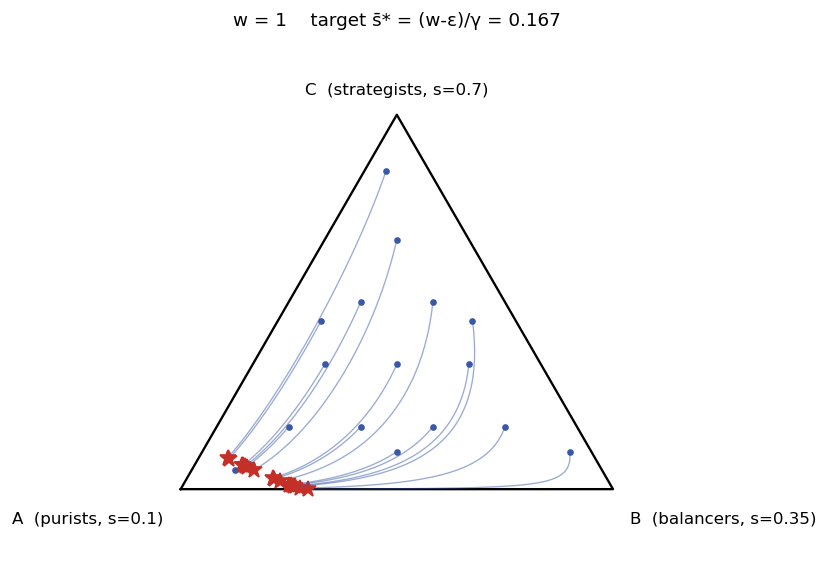
\includegraphics[width=0.75\textwidth]{simplex_w1.png}
  \caption{Phase portrait on $\Delta^2$ at $w = 1$ (below threshold).
    A- and C-vertices are unstable sources and B is a saddle; no
    corner is an ESS. Trajectories settle on or near the A--B edge,
    consistent with the continuous-game rest point
    $s^\ast = (w - \varepsilon)/\gamma = 0.167$. Integrated by forward
    Euler ($\Delta t = 0.05$, $T = 200$) from a grid of 30 interior
    starting points; blue dots mark initial conditions, red stars mark
    trajectory end-points.}
  \label{fig:simplex_w1}
\end{figure}

\begin{figure}[H]
  \centering
  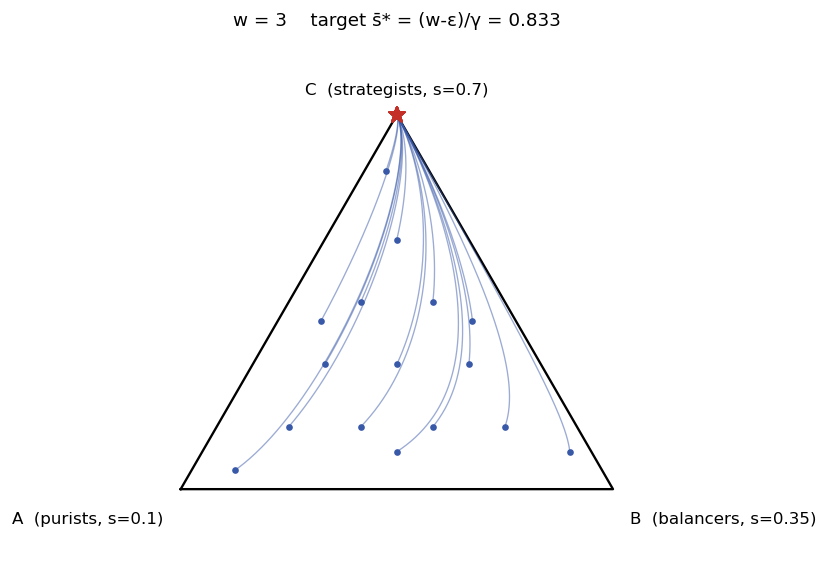
\includegraphics[width=0.75\textwidth]{simplex_w3.png}
  \caption{Phase portrait on $\Delta^2$ at $w = 3$ (above threshold
    $w^\ast = 2.60$). The C-vertex is the unique stable strict ESS;
    all 30 interior trajectories converge to it. Markers and
    integration scheme as in Figure~\ref{fig:simplex_w1}.}
  \label{fig:simplex_w3}
\end{figure}

\begin{figure}[H]
  \centering
  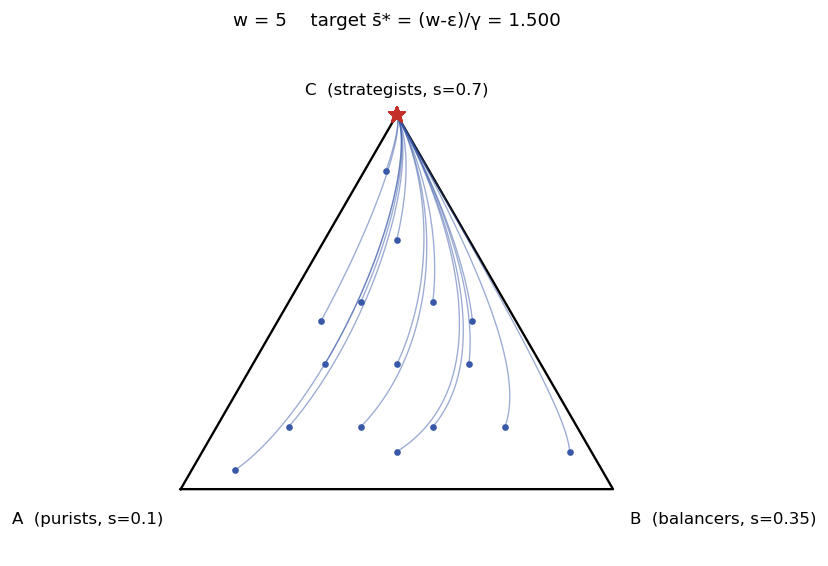
\includegraphics[width=0.75\textwidth]{simplex_w5.png}
  \caption{Phase portrait on $\Delta^2$ at $w = 5$. The C-vertex
    remains the unique stable strict ESS, with more negative invasion
    eigenvalues and visibly faster convergence than at $w = 3$.
    Markers and integration scheme as in Figure~\ref{fig:simplex_w1}.}
  \label{fig:simplex_w5}
\end{figure}

\subsection{Survey Data}
\label{sec:data}

We administered a Google Form survey to $n = 42$ Dartmouth
undergraduates during Spring term 2026, with the form distributed
through classmates and peer networks. The
sample skews toward Finance/consulting ($n = 24$, 57\%) and Economics
majors ($n = 14$, 33\%). The mean GPA-importance rating is
$\bar{w} = 3.57$ on a 1--5 scale. The distribution of $s$ is
right-skewed, with most respondents between 0--40\% layups and a
smaller tail above 50\%. Mean layup ratios range from
$\bar{s} = 0.100$ (pre-medical) to $\bar{s} = 0.350$
(finance/consulting). Figure~\ref{fig:desc} gives the full descriptive
overview.

\begin{figure}[H]
  \centering
  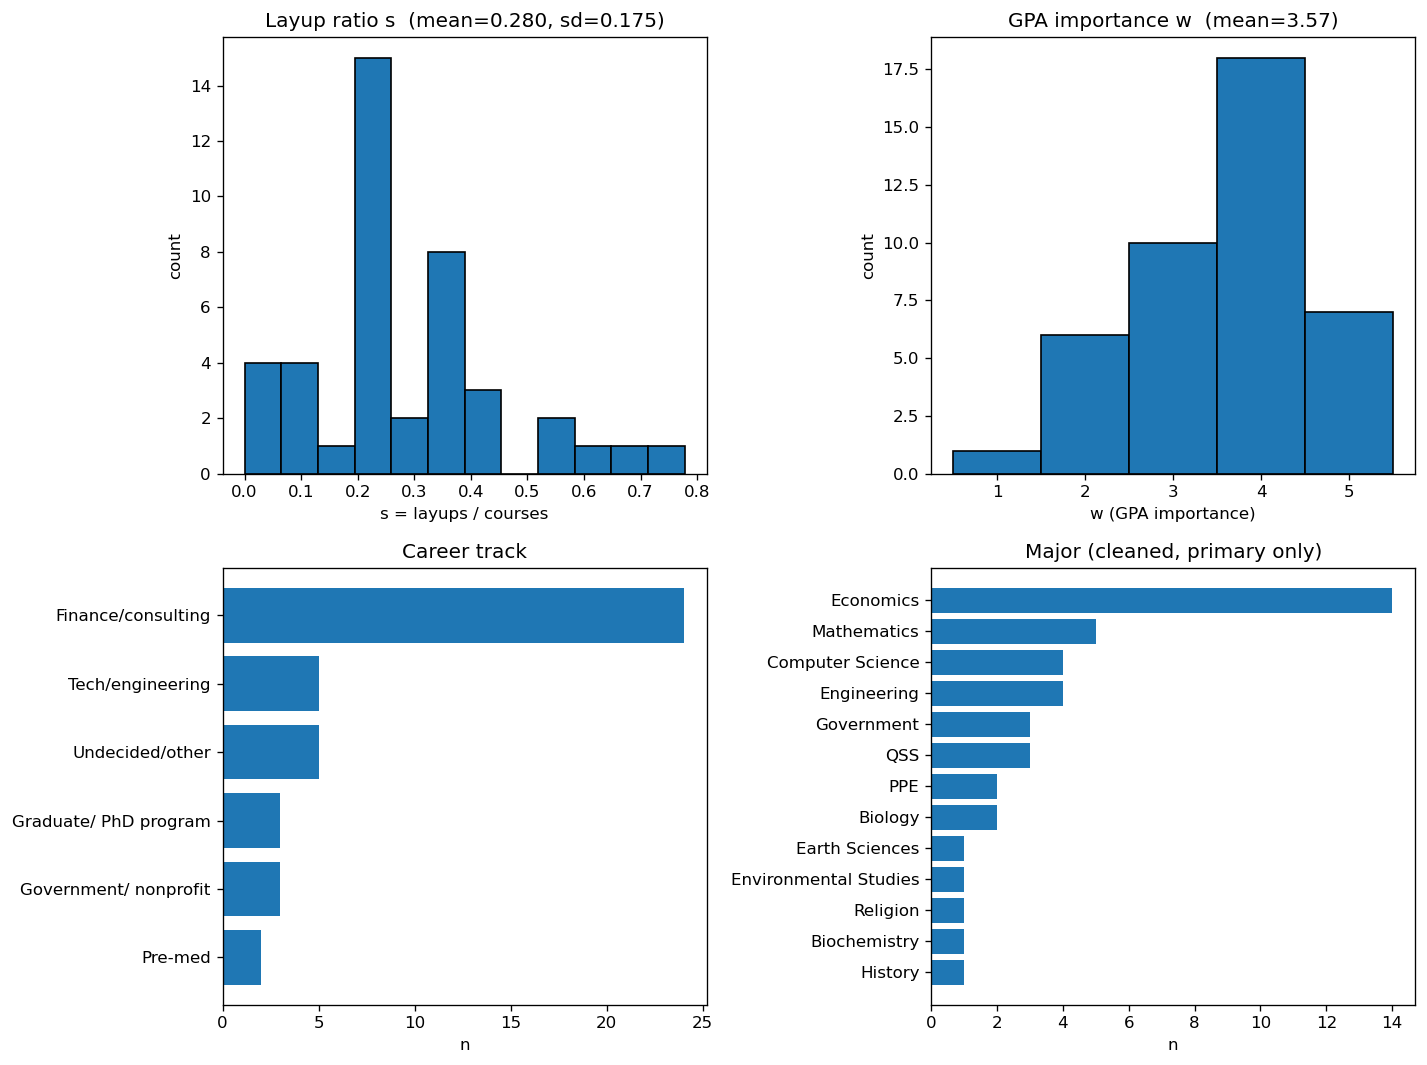
\includegraphics[width=0.85\textwidth]{desc_overview.png}
  \caption{Survey sample ($n = 42$). Top row: distribution of layup
    ratio $s$ (left) and GPA-importance rating $w$ (right). Bottom
    row: composition by career track and major. Finance/consulting
    and Economics are over-represented.}
  \label{fig:desc}
\end{figure}

\subsection{P1: GPA Importance and Layup Ratio}

The model predicts $\partial s^\ast / \partial w = 1/\gamma > 0$. We
test with OLS,
\begin{equation}
  s_i = \alpha + \beta_w\, w_i + \bm{\delta}_{\text{year}} +
        \bm{\delta}_{\text{major}} + \varepsilon_i,
\end{equation}
with year and major indicator controls and HC1 standard errors
\parencite{long2000using}. The estimate is $\hat\beta_w = +0.0103$
(95\% CI $[-0.083, +0.103]$, $p = 0.83$). The sign matches the
prediction, but the effect is statistically indistinguishable from
zero, and with 16 fixed-effect indicators on $n = 42$ the
specification is over-parameterized (adjusted $R^2 = -0.246$), so the
slope is heavily attenuated. Treating the
(statistically insignificant) point estimate as if it were identified,
inverting $\bar s^\ast = (w - \varepsilon)/\gamma$ gives an implied
$\hat\gamma = 1/\hat\beta_w \approx 97$. Because the 95\% CI for
$\beta_w$ includes zero, this implied $\hat\gamma$ is unbounded above
and is not a formal estimate; we report it only as a directional check
that the calibrated $\gamma = 3$ likely understates peer-level
competition. Dropping the six double-major
respondents leaves the sign unchanged
($\hat\beta_w = +0.051$, $p = 0.47$).

\subsection{P2: Cross-Track Distribution of Layup Ratios}

We regress $s_i$ on career-track indicators with Undecided/other as
the baseline (HC1 errors). The overall $F$-test rejects homogeneity
($F = 3.13$, $p = 0.019$), but Table~\ref{tab:track} shows the
ordering is not what the model predicts. Finance/consulting ranks
highest ($\bar s = 0.350$), followed by Government/nonprofit (0.233),
Tech/engineering (0.220), Undecided/other (0.183), Graduate/PhD
(0.148), and Pre-medical (0.100). Pre-medical students, whom the
model identifies as the most strategic (highest mean $w = 4.5$,
$n = 2$), exhibit the \emph{lowest} observed layup ratio. Only the
Finance/consulting coefficient is significant against the baseline
($\hat\beta = +0.167$, $p = 0.012$); see Figure~\ref{fig:p2}.

\begin{table}[H]
\centering
\caption{Track-level statistics, sorted by mean layup ratio.
$\hat\beta$ and $p$-value are OLS coefficients relative to
Undecided/other, HC1 standard errors. The Pre-medical SD ($n = 2$)
is mechanically $|x_1 - x_2|/\sqrt{2}$ and carries no inferential
content.}
\label{tab:track}
\small
\begin{tabular}{lcccrc}
\toprule
Track & $n$ & $\bar{s}$ & $\text{SD}(s)$ & $\hat{\beta}$ & $p$ \\
\midrule
Finance/consulting   & 24 & 0.350 & 0.167 & $+0.167$ & 0.012 \\
Government/nonprofit &  3 & 0.233 & 0.096 & $+0.050$ & 0.505 \\
Tech/engineering     &  5 & 0.220 & 0.204 & $+0.037$ & 0.724 \\
Undecided/other      &  5 & 0.183 & 0.130 & (baseline) & n/a \\
Graduate/PhD program &  3 & 0.148 & 0.128 & $-0.035$ & 0.683 \\
Pre-medical          &  2 & 0.100 & 0.141 & $-0.083$ & 0.379 \\
\bottomrule
\end{tabular}
\end{table}

\begin{figure}[H]
  \centering
  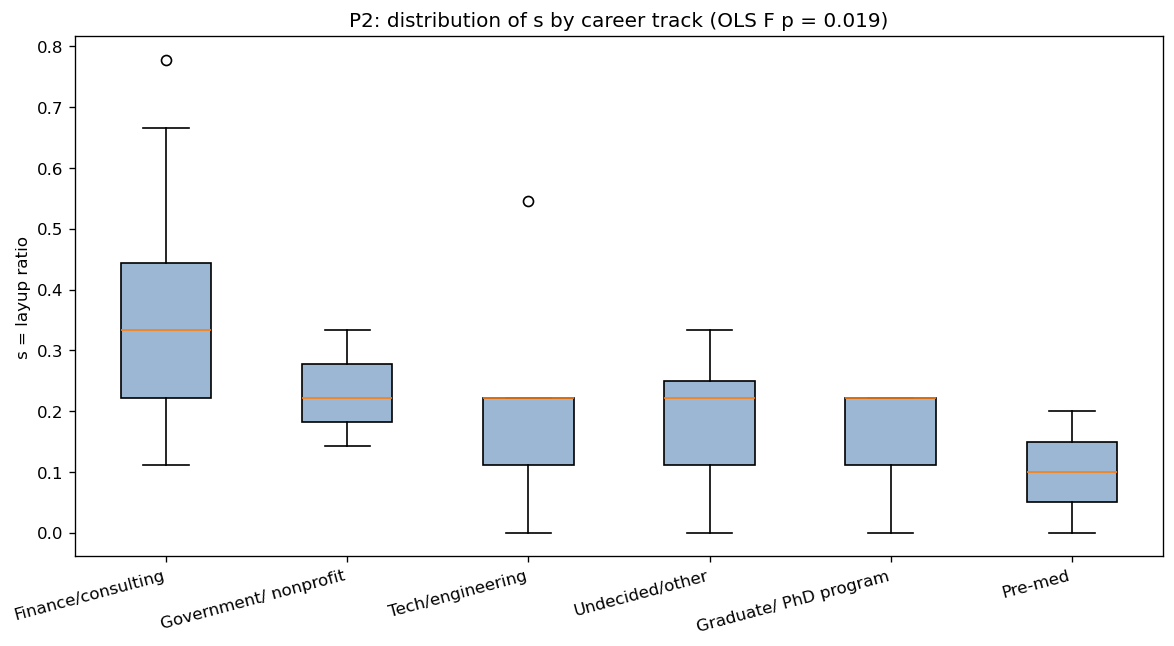
\includegraphics[width=0.7\textwidth]{p2_box_s_by_track.png}
  \caption{Distribution of layup ratio $s$ by career track (descending
    means). Boxes span the interquartile range. The overall $F$-test
    rejects homogeneity ($F = 3.13$, $p = 0.019$). Contrary to the
    model, Pre-medical students show the lowest mean.}
  \label{fig:p2}
\end{figure}

\subsection{P3 and P4: GPA-Protective Avoidance and Peer Pressure}

For P3, respondents reporting course avoidance at least once
(Q7 $\geq 1$, $n = 18$) show slightly higher $s$ and $w$ than those
who never avoided ($n = 24$). The differences are
$E[s\mid\text{avoided}] - E[s\mid\text{never}] = +0.038$ and
$E[w\mid\text{avoided}] - E[w\mid\text{never}] = +0.361$, both with
the predicted sign but not significant (one-sided Mann--Whitney
$p = 0.17$ for both).

For P4, Q9 asked whether the Dartmouth environment pushes students
toward easy courses on a $-2$ to $+2$ scale. The Spearman correlation
between Q9 and $s$ is $\hat\rho = +0.231$ (one-sided $p = 0.07$;
two-sided $p = 0.14$; $n = 42$), a small positive association in the
predicted direction. Figure~\ref{fig:p4} shows the scatter with horizontal
jitter for legibility.

\begin{figure}[H]
  \centering
  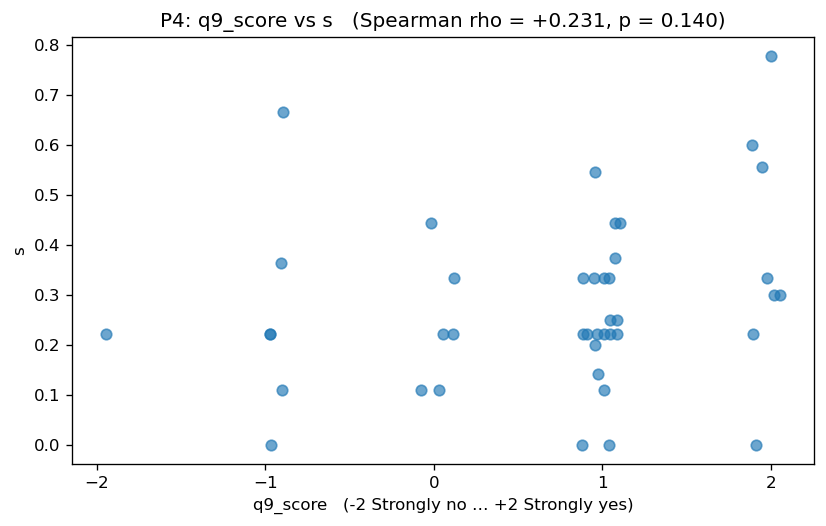
\includegraphics[width=0.55\textwidth]{p4_scatter_q9_s.png}
  \caption{Scatter of $s$ against perceived environmental pressure
    toward easy courses (Q9 score, with horizontal jitter).
    Spearman $\hat\rho = +0.231$ ($p = 0.14$, $n = 42$).}
  \label{fig:p4}
\end{figure}

\subsection{Empirical Simplex Overlay}

We classify each respondent as type $A$ if $s < 0.20$, type $B$ if
$0.20 \leq s < 0.50$, or type $C$ if $s \geq 0.50$ (cutoffs are
rounded midpoints between adjacent type values $s_A, s_B, s_C$), then
compute the empirical type distribution $(x_A, x_B, x_C)$ within each
track and plot the result on $\Delta^2$ (Figure~\ref{fig:simplex_emp}). Every
track clusters in the B-vertex region. Finance/consulting, the track
with the highest mean $s$, still has only 17\% strategists and 75\%
balancers; every other track has zero strategists. The model,
calibrated at $\gamma = 3.0$ and evaluated at $\bar w = 3.57$,
predicts convergence to the C-vertex. The data show the opposite.
This discrepancy is our most substantive empirical finding.

\begin{figure}[H]
  \centering
  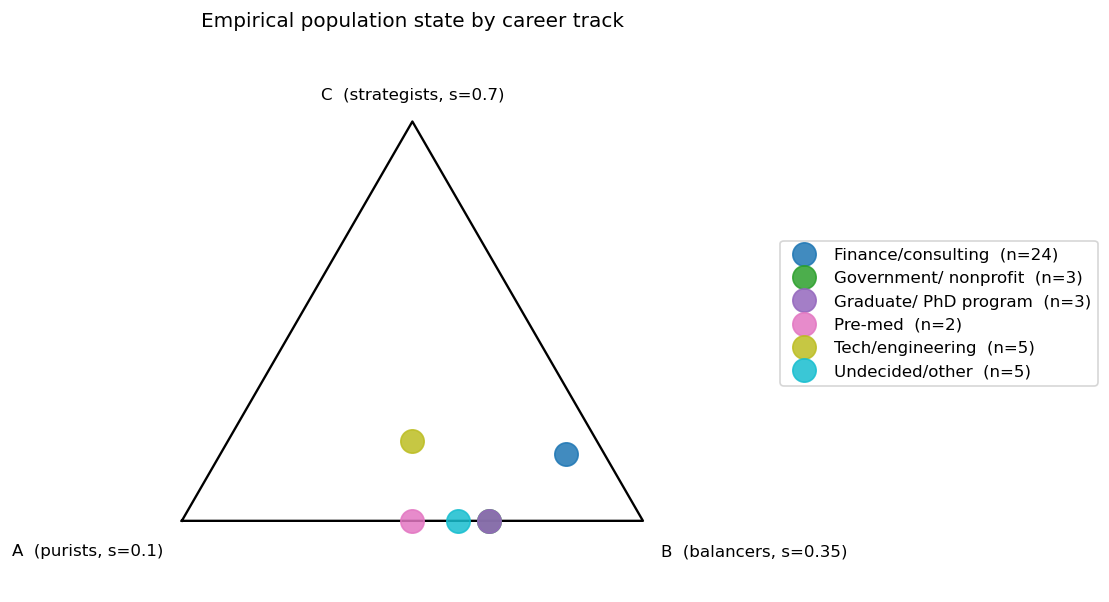
\includegraphics[width=0.6\textwidth]{empirical_simplex.png}
  \caption{Empirical population state by career track on $\Delta^2$
    (type defined by layup ratio). Every track clusters near the
    B-vertex, contrary to the model's prediction of C-vertex
    dominance at $\bar w = 3.57$.}
  \label{fig:simplex_emp}
\end{figure}

\subsection{Policy Counterfactual: Eliminating Enforced Grading Medians}

Many Dartmouth departments enforce grading medians, which fix the
share of A-level grades and so make each student's payoff highly
sensitive to peer enrollment, since one student's A displaces
another's. Removing this cap loosens the coupling between individual
payoff and aggregate behavior, which we model as a reduction in
$\gamma$ from 3 to 1.5. The opposite reading, that medians blunt the
upside of grade-seeking and their removal raises $\gamma$, is also
defensible; we therefore treat the direction as a modeling assumption
rather than a derivation, and report the counterfactual conditional on
it.
Under the replicator dynamics, the target layup ratio
$\bar s^\ast = (w - \varepsilon)/\gamma$ doubles for any $w$
(Table~\ref{tab:policy}). For $w \geq 3$, the baseline target already
exceeds $s_C$ and the equilibrium is pinned at the C-vertex regardless.
The implication is troubling. Eliminating enforced medians raises the
equilibrium layup ratio precisely for low-to-moderate-$w$ students,
the group reformers might most hope to redirect toward substantive
coursework.

\begin{table}[H]
\centering
\caption{Median-elimination counterfactual ($\gamma \to \gamma/2 = 1.5$)
on $\bar s^\ast = (w - \varepsilon)/\gamma$, capped at $1.0$.}
\label{tab:policy}
\small
\begin{tabular}{cccc}
\toprule
$w$ & $\bar{s}^*$ ($\gamma = 3$) & $\bar{s}^*$ ($\gamma = 1.5$) & $\Delta \bar{s}^*$ \\
\midrule
1 & 0.167 & 0.333 & $+0.167$ \\
2 & 0.500 & 1.000 & $+0.500$ \\
3 & 0.833 & 1.000 & $+0.167$ \\
4 & 1.000 & 1.000 & 0.000 \\
5 & 1.000 & 1.000 & 0.000 \\
\bottomrule
\end{tabular}
\end{table}

% ============================================================
\section{Methods}
% ============================================================

\paragraph{Survey and variables.}
A Google Form survey was administered to Dartmouth undergraduates
during Spring term 2026, with the form link distributed through
classmate and peer-network outreach. Inclusion required current
enrollment and at least one prior on-campus term. The form defined a
layup as a course taken primarily for its expected grade rather than
its content, and respondents self-counted using that definition.
Respondents reported class year, primary major, intended career track,
counts of total and layup courses over the three most recent on-campus
terms, whether they had ever avoided a course to protect GPA, GPA
importance on a 1--5 scale, and perceived environmental pressure
toward easy courses. The
final sample is $n = 42$, with all respondents reporting complete
layup and course-count fields (no rows were dropped). The layup ratio
is $s_i = \text{layups}_i / \text{courses}_i \in [0, 1]$.
GPA importance $w_i$ maps to $\{1, \dots, 5\}$. Course avoidance (Q7)
maps to $\{0, 1, 2\}$, dichotomized at Q7 $\geq 1$ for P3. Perceived
pressure $q9_i$ maps to $\{-2, \dots, +2\}$. Majors are normalized to
the primary major only, with a binary double-major flag for robustness
checks.

\paragraph{Model parameterization.}
The type-specific ratios $s_A = 0.10$, $s_B = 0.35$, $s_C = 0.70$ span
the empirical range of $s$ and demarcate minimal, moderate, and heavy
layup-taking. The baseline value $\varepsilon = 0.5$ reflects the
assumption that a non-layup course retains substantial value without
competition. The competition intensity $\gamma = 3.0$ was calibrated
so the continuous-game attractor $s^\ast = (w - \varepsilon)/\gamma$
lies between the purist and strategist ratios,
$s_A < s^\ast < s_C$, over $w \in (0.8, 2.6)$, keeping the replicator
dynamics non-trivially interior across the lower half of the survey's
$w$ range.

\paragraph{Simulation and statistics.}
\label{sec:sim}
The replicator dynamics (Eq.~\ref{eq:replicator}) were integrated by
forward Euler on $\Delta^2$ with $\Delta t = 0.05$ and $T = 200$. After
each step, $\bm{x}$ was clipped to $[10^{-12}, 1]$ componentwise and
re-normalized. Vertex stability was computed analytically using
Eq.~\ref{eq:invasion}, which gives the two non-trivial tangent-space
eigenvalues directly and avoids the spurious off-simplex eigenvalue
of a naive 3D finite-difference Jacobian. P1 and P2 use OLS with HC1
standard errors \parencite{long2000using}. Although $s_i$ is bounded
and ratio-valued, OLS is used for interpretability and ease of HC1
inference; given the small sample, we do not pursue a fractional-logit
specification. P3 uses a one-sided Mann--Whitney $U$ test, suited to
small unequal groups. P4 uses
Spearman's $\rho$ (reported one-sided, given the directional
prediction) because $q9$ is ordinal. Analyses were run in
Python 3.13.

% ============================================================
\section{Discussion}
\label{sec:discussion}
% ============================================================

\subsection{Summary}

We introduced a three-type replicator model of course selection in
which payoffs depend on the collective layup intensity through a
competition parameter $\gamma$. The strategist equilibrium is locally
stable once $w > 2.60$ under our calibration, and numerical
integration from a grid of interior initial conditions suggests it
also attracts globally in this regime.
Against 42 survey responses, three of the four directional predictions
(P1, P3, P4) hold in sign but fall short of conventional significance;
P2's cross-track $F$-test rejects homogeneity ($p = 0.019$), but the
predicted ordering does not hold. Two substantive anomalies stand out,
the pre-medical reversal and the population's concentration at the
B-vertex.

\subsection{Empirical Anomalies}

\textit{The pre-medical reversal.}
Pre-medical students confirm the first half of the model
($\bar w = 4.5$) but contradict the second ($\bar s = 0.100$, lowest
of any track). With $n = 2$, no inference about the group mean is
warranted. The more substantive possibility is that pre-meds use a
different GPA-protective strategy. Rather than padding their
transcript with known layups, they may avoid difficult courses
altogether, curating a schedule of moderately rigorous but manageable
classes. The relevant strategy axis would then be expected course
difficulty, not layup fraction. Pre-meds minimize difficulty through
selection-out rather than selection-in. Course-difficulty ratings (for
example, from online platforms or faculty grade distributions) would
let future work model this directly.

\textit{The B-vertex puzzle.}
With mean $\bar w = 3.57$ above the threshold $w = 2.60$, the
model predicts universal convergence to strategist dominance, yet the
empirical population sits firmly in the balancer region. Three
explanations are plausible, and they likely operate together. First,
$\gamma$ may be substantially higher than the calibrated 3. The small
observed slope $\hat\beta_w \approx 0.01$ is mechanically consistent
with very large $\gamma$ (the inverted point estimate
$1/\hat\beta_w \approx 97$ is formally unidentified given the
insignificant slope), and any $\gamma$ above roughly 9 pushes the
C-vertex stability threshold $w^\ast = \gamma s_C + \varepsilon$ above
the observable $w$ range, removing the strict prediction of strategist
dominance. High $\gamma$ on its own would, however, drive the dynamics
toward the A-vertex rather than the B-vertex, since
$s^\ast = (w - \varepsilon)/\gamma$ falls below $s_A$ for large
$\gamma$; the level concentration at B must therefore come from
something beyond the calibrated competition channel. Second, the
model omits fitness costs of extreme strategist behavior, including
reputation effects with faculty, advising constraints, and intrinsic
preferences for learning. These costs penalize the C-corner and could
stabilize an interior region around B. Third, the sample
over-represents Economics and Finance/consulting students, whose
disciplinary norms may suppress extreme layup-taking.

\subsection{Policy Implications and Coupled Dynamics}

Our counterfactual is cautionary for institutional reformers.
Eliminating enforced grading medians is often proposed on the
intuition that reduced competitive pressure will move students toward
challenging courses. The model says the opposite. Reducing $\gamma$
raises the equilibrium target $\bar s^\ast$ for low-to-moderate-$w$
students, the very group reformers most hope to redirect. This is a
version of the collective-action failure identified by
\textcite{bok2006underachieving}: interventions that reduce the
\emph{cost} of strategic behavior may encourage it.

A deeper limitation is that the counterfactual treats $\gamma$ as
exogenous. Grade inflation is itself the outcome of accumulated
strategic course selection. As $\bar s$ rises and students
concentrate in high-median courses, the grade distribution compresses
and the marginal payoff to another layup shifts. This is a textbook
case of coupled environment--strategy dynamics
\parencite{weitz2016oscillating, tilman2020evolutionary}. A complete
model would couple the replicator equation to an environmental
variable $n$ representing grading stringency,
\begin{equation}
  \dot{\bar s} = \tau_s\, \bar s (1 - \bar s)\,\Delta f(n),
  \qquad
  \dot n = \tau_n\bigl[g(n) - h(\bar s, n)\bigr],
\end{equation}
where $\tau_s, \tau_n$ are time-scale parameters, $\Delta f(n)$ is the
payoff differential as a function of stringency, and $g, h$ capture
how collective layup-taking erodes grading discipline. Such systems can produce persistent oscillations
between ``conservation'' and ``exploitation'' regimes that no
decoupled replicator model can capture. The multi-decade decline in
study time documented by \textcite{babcock2011falling} is
qualitatively consistent with the descending arc of such a cycle.
Institutional reforms act primarily on the $n$-dynamics, not on
$\gamma$ directly, which makes the decoupled counterfactual a
conservative guide.

\paragraph{Limitations and future directions.}
The sample ($n = 42$) is a single-institution convenience sample
drawn through the authors' peer networks, with no random selection
and all key variables self-reported; the resulting skew toward
Finance/consulting and Economics is the most visible expression of
this design limitation. The parameters $\gamma$ and $\varepsilon$ are
calibrated rather than estimated. Future work should pursue
transcript-level data (enabling structural estimation of $\gamma$),
multi-institution comparisons (Princeton's 2004 grade-deflation
policy offers exogenous variation in $\gamma$), and a richer strategy
space with course difficulty as a continuous dimension and
heterogeneous $w$.

% ============================================================
\printbibliography[title={References}]
% ============================================================

\end{document}
